% experiments.tex — experiments section (draft 2026-09-16; RAW, not jointly agreed). \input from
% iclr2027_conference.tex. Tables and the thickness theory are Berker's, unchanged except the two
% corrected table cells (S-400 linear 72.2; video B-240 CLS 42.2). Details: experiments_details.tex.
\section{Experiments}
\label{sec:experiments}

\subsection{Setup and datasets}
\label{sec:exp-setup}
We use ImageNet-1k for large-scale image SSL, ImageNet-100 for controlled experiments, and Kinetics-710 for video, where we follow LeVJEPA and train on a class-balanced 20\% subset. The controlled experiments use ViT-S. The large-scale runs use ViT-S and ViT-B for 100 and 400 epochs on images, and up to 1{,}085 epochs on video, to show that the method is also suitable for longer training. Due to compute limitations these are single runs without hyperparameter tuning, so the reported numbers are likely below what the method can reach. For evaluation we follow the standard frozen-feature protocols: the linear-probe and kNN protocol of the Lightly benchmark on ImageNet-1k, the VISReg protocol for transfer, and the LeVJEPA protocol for video; details are given in Appendix~\ref{app:exp-details}. Whenever public checkpoints trained under one codebase are available (OK-AI), we evaluate them under the same protocol; otherwise we report the published numbers.
% TODO cite: CMC (ImageNet-100), OK-AI, Lightly benchmark, LeVJEPA.

\subsection{ImageNet-1k with ViT-S and ViT-B at 100 and 400 epochs}
\label{sec:exp-in1k}
% Sources: results/probes/*.bench{,_knn}.csv, results/transfer/*.visreg_lp.csv (E27 card).
Table~\ref{tab:in1k-main} reports linear-probe and kNN accuracy on ImageNet-1k, and Table~\ref{tab:transfer-main} the average transfer accuracy over eight classification datasets. Used as a standalone method, with the regularizer applied both at the backbone and after the projector, our objective is competitive with the strongest epoch-matched baselines. On the linear probe, ViT-S is within 0.3 points of DINO at 100 epochs and 1.6 points below its 300-epoch checkpoint at 400 epochs, and ViT-B lies between DINO and iBOT at both training lengths. On transfer our models match or exceed every epoch-matched baseline at 100 epochs, including iBOT, and stay within 0.3 points of iBOT at longer training; the published 400-epoch DINO and iBOT checkpoints remain about one point ahead. kNN accuracy is where we are weakest, 5 to 9 points below DINO and iBOT. Training for 400 instead of 100 epochs improves linear and transfer accuracy at both model sizes, so the method keeps improving with longer training.

\subsection{Beyond image SSL: the recipe on video}
\label{sec:exp-video}
% Sources: E34 card (§B ladder, §K400 feature read); D-124 as amended.
We apply the same objective to video by replacing the loss inside the LeVJEPA training pipeline and keeping their model, optimizer and data pipeline. Frozen encoders are evaluated on three benchmarks that test different content: ImageNet-1k (a single image; appearance), Something-Something-v2 (short clips of human--object interactions such as \emph{putting something into something}, where the label is the temporal relation), and Kinetics-400 (short real-world clips such as \emph{playing guitar}; appearance and context). Table~\ref{tab:video-main} compares our ViT-S at 240 epochs and ViT-B at 240 and 1{,}085 epochs with LeVJEPA, V-JEPA~2 and VideoMAEv2 at matched epochs. On ImageNet-1k our encoders are ahead of LeVJEPA and V-JEPA~2 at 240 epochs for both sizes; at 1{,}085 epochs we stay below LeVJEPA and above the other two. The largest effect is on the temporal benchmark: on SSv2 our ViT-B is 13.5 points above LeVJEPA at 240 epochs and 7.9 points above its 1{,}085-epoch model, and ahead of V-JEPA~2 and VideoMAEv2 as well. On Kinetics-400 we are within 1.2 points of LeVJEPA with the same mean-pooled linear probe; since LeVJEPA does not release its probe settings, we also report the linear probe on the CLS token and the attentive probe.
% TODO cite: LeVJEPA, V-JEPA 2, VideoMAEv2, SSv2, Kinetics.

\subsection{Controlled experiments on ImageNet-100: the regularizer on other methods}
\label{sec:exp-in100}
% Sources: results/probes/<run>.csv; results/compare/e20_battery_vs_ctrl.csv; thm21_exhibit.csv;
% E20 card (dose rule, E20-T1..T4 agreed); E29 (VISReg pair); E33-T1 agreed (D-113).
The large-scale runs use the regularizer in both spaces. To isolate its effect at the backbone, we train six augmentation-based methods on ImageNet-100 (LeJEPA, VICReg, SimCLR, DINO, BYOL, VISReg) with their own objectives, and once more with $\beta_{\mathrm{reg}}\mathcal{R}_{\mathrm{KL}}$ added at the backbone and everything else unchanged. The weight is not tuned per method: it is set so that the added term contributes a fixed small fraction of the gradient on the backbone (Appendix~\ref{app:exp-details}). Our own objective is included with and without the backbone term.

Figure~\ref{fig:constraint-mismatch} confirms on these models what Section~\ref{sed:related_work} argued: each method's own constraint holds after the projector and not at the backbone (LeJEPA's Gaussianity, VICReg's variance criterion, SimCLR's alignment). Figure~\ref{fig:two-space-audit} shows what the backbone regularizer changes. At the backbone, the effective rank rises from 6--24\% of the feature dimension to 51--86\%, and the rank of the between-image covariance rises with it; after the projector the same statistics barely move. Downstream performance follows the backbone, not the loss space: kNN accuracy improves for every method, by 3 to 13 points, and linear-probe accuracy improves for all but VICReg, where it is unchanged. Figure~\ref{fig:rich-learning} shows that this capacity is not obtained by freezing feature learning: the backbone features move far from their initialization and the tangent kernel keeps changing during training, as for the unregularized model.

\subsection{Augmentation thickness}
\label{sec:exp-thickness}
Let $Q$ denote the source image and let $H$ vary over augmented views of $Q$. We decompose its covariance into

\begin{equation}
    C_h = B_h + A_h,
    \qquad
    B_h = \operatorname{Cov}\!\left(\mathbb{E}[H \mid Q]\right),
    \qquad
    A_h = \mathbb{E}\!\left[\operatorname{Cov}(H \mid Q)\right].
\end{equation}
Here, $B_h$ measures variation between images, while $A_h$ measures variation across views of the same image. $A_h$ alone is difficult to interpret: the same amount of view variation matters differently when image centers are well separated or concentrated. We therefore measure augmentation variation relative to between-image variation and define

\begin{equation}
    \Theta_h
    =
    B_h^{\dagger/2} A_h B_h^{\dagger/2}.
    \label{eq:thickness}
\end{equation}
Along any direction $a$ with nonzero between-image variance,

\begin{equation}
    \theta_h(a)
    =
    \frac{a^\top A_h a}{a^\top B_h a}.
\end{equation}
We call $\Theta_h$ the \emph{augmentation thickness} of the retained representation.

Thickness is not a quantity that should simply be minimized. Consider a centered image-level target $y$ with $\|y\|_{L_2}\leq1$. Let
\begin{equation}
    E_{\mathcal A}(y)
    =
    \min_f
    \mathbb{E}\!\left[(y(Q)-f(V))^2\right]
\end{equation}

% be the best possible prediction error for $y$ from a single augmented view
be the irreducible error of predicting $y$ from a single augmented view, and let $d_h(y)$ be the error of the best linear prediction from the backbone image centers.

\begin{theorem}[Two sides of augmentation thickness]
\label{thm:thickness}
Assume the image-center covariance is whitened. Then,
\begin{equation}
    d_h(y)
    \geq
    \left(
        \sqrt{E_{\mathcal A}(y)}
        -
        \sqrt{\|\Theta_h\|_{\mathrm{op}}}
    \right)_+ .
    \label{eq:too-thin}
\end{equation}
% Moreover, let $a^\top m_h(Q)$ be the best linear prediction of $y$ from the image centers. Then the best linear prediction error from a single view representation $H$ is
Moreover, let $a$ be the coefficient vector of the best linear prediction of $y$ from the image centers. Then the best linear prediction error from a single view representation $H$ is
\begin{equation}
    \inf_u
    \mathbb{E}\!\left[(y-u^\top H)^2\right]
    =
    d_h(y)^2
    +
    a^\top
    \Theta_h (I+\Theta_h)^{-1} a.
    \label{eq:too-thick}
\end{equation}
For fixed image-center organization and task direction, this error term increases as augmentation thickness increases.
\end{theorem}

The proof is given in Appendix~\ref{app:thickness}. The first result shows that making $H$ too invariant can remove differences between images that are affected by the augmentations. The second shows that, for the same organization across image centers, more variation across views makes prediction from a view harder. Thus, thickness captures a trade-off: we do not want to remove all augmentation variation, but we also do not want it to dominate the representation.
\paragraph{Thickness and the regularizer.}
% Sources: results/diag/e23_retro_spaces.csv (Theta_h per model); C8 (fig_org_vs_sensitivity,
% agreed 2026-08-13); E36 card (the centroid vs residual split, RAW).
We estimate $\Theta_h$ from eight augmented views per image (Appendix~\ref{app:exp-details}). Figure~\ref{fig:thickness-gain} places every ImageNet-100 model in the plane of thickness and accuracy: the backbone regularizer makes $h$ thicker for every method, and accuracy rises at the same time, so the gain is not obtained by making the retained representation more invariant. Figure~\ref{fig:organization-sensitivity} looks at the same models through Eq.~\eqref{eq:too-thick}, per class: with the regularizer, the view-sensitivity term along the class direction grows slightly while the organization of the image centers improves more, so the single-view error falls (for 96 of 100 classes in our model). The regularized backbone therefore keeps more augmentation-dependent variation along class directions, and its accuracy gain comes from better organized image centers rather than from that variation.

\begin{table}[h]
\centering
\small
\begin{tabular}{llrrr}
\toprule
Method & Backbone & Ep. & Linear & kNN \\
\midrule
LeJEPA (OK-AI) & ViT-S/16 & 100 & 62.5 & 45.5 \\
DINO (OK-AI) & ViT-S/16 & 100 & 70.0 & 64.7 \\
iBOT (OK-AI) & ViT-S/16 & 100 & 70.9 & 65.7 \\
\textbf{Ours} & \textbf{ViT-S/16} & \textbf{100} & \textbf{69.7} & \textbf{59.2} \\
\midrule
LeJEPA (OK-AI) & ViT-S/16 & 300 & 66.4 & 51.5 \\
DINO (OK-AI) & ViT-S/16 & 300 & 73.8 & 71.0 \\
iBOT (OK-AI) & ViT-S/16 & 300 & 75.2 & 71.5 \\
\textbf{Ours} & \textbf{ViT-S/16} & \textbf{400} & \textbf{72.2} & \textbf{62.9} \\
\midrule
LeJEPA (OK-AI) & ViT-B/16 & 100 & 69.7 & 51.3 \\
DINO (OK-AI) & ViT-B/16 & 100 & 73.9 & 69.4 \\
iBOT (OK-AI) & ViT-B/16 & 100 & 77.0 & 72.9 \\
VISReg (repro.) & ViT-B/16 & 100 & 70.3 & 52.5 \\
\textbf{Ours} & \textbf{ViT-B/16} & \textbf{100} & \textbf{74.2} & \textbf{64.3} \\
\midrule
LeJEPA (OK-AI) & ViT-B/16 & 300 & 72.4 & 59.4 \\
DINO (OK-AI) & ViT-B/16 & 300 & 75.2 & 73.5 \\
iBOT (OK-AI) & ViT-B/16 & 300 & 78.6 & 77.0 \\
MoCo v3 & ViT-B/16 & 300 & 75.9 & 68.2 \\
DINO & ViT-B/16 & 400 & 77.2 & 73.3 \\
iBOT & ViT-B/16 & 400 & 78.5 & 74.8 \\
VISReg & ViT-B/16 & 400 & 74.6 & 60.0 \\
\textbf{Ours} & \textbf{ViT-B/16} & \textbf{400} & \textbf{76.0} & \textbf{68.6} \\
\bottomrule
\end{tabular}
\caption{ImageNet-1k linear-probe and kNN ($k{=}200$) top-1 accuracy (\%) under one protocol for every row (Section~\ref{sec:exp-setup}). OK-AI rows are public checkpoints of one codebase at 100 and 300 epochs; VISReg (repro.) is the authors' code run end-to-end by us for 100 epochs; the 300/400-epoch public checkpoints are context. Our ViT-S/16 at 400 epochs is the run described in Appendix~\ref{app:exp-details}.}
% RAW (not jointly agreed). Source: results/probes/<rid>.bench.csv (max over 90 epochs) + .bench_knn.csv (t=.07); generator experiments/paper_exhibits.py::comparison_tables().
\label{tab:in1k-main}
\end{table}

\begin{table}[t]
\centering
\small
\begin{tabular}{llrr}
\toprule
Method & Backbone & Ep. & Transfer Avg. \\
\midrule
LeJEPA (OK-AI) & ViT-S/16 & 100 & 68.7 \\
DINO (OK-AI) & ViT-S/16 & 100 & 75.7 \\
iBOT (OK-AI) & ViT-S/16 & 100 & 75.9 \\
\textbf{Ours} & \textbf{ViT-S/16} & \textbf{100} & \textbf{77.6} \\
\midrule
LeJEPA (OK-AI) & ViT-S/16 & 300 & 71.9 \\
DINO (OK-AI) & ViT-S/16 & 300 & 79.4 \\
iBOT (OK-AI) & ViT-S/16 & 300 & 79.5 \\
\textbf{Ours} & \textbf{ViT-S/16} & \textbf{400} & \textbf{79.3} \\
\midrule
LeJEPA (OK-AI) & ViT-B/16 & 100 & 74.2 \\
DINO (OK-AI) & ViT-B/16 & 100 & 78.3 \\
iBOT (OK-AI) & ViT-B/16 & 100 & 80.7 \\
VISReg (repro.) & ViT-B/16 & 100 & 76.4 \\
\textbf{Ours} & \textbf{ViT-B/16} & \textbf{100} & \textbf{80.9} \\
\midrule
LeJEPA (OK-AI) & ViT-B/16 & 300 & 75.2 \\
DINO (OK-AI) & ViT-B/16 & 300 & 79.3 \\
iBOT (OK-AI) & ViT-B/16 & 300 & 82.3 \\
MoCo v3$^\ddag$ & ViT-B/16 & 300 & 80.5 \\
DINO$^\ddag$ & ViT-B/16 & 400 & 83.1 \\
iBOT$^\ddag$ & ViT-B/16 & 400 & 83.2 \\
VISReg$^\ddag$ & ViT-B/16 & 400 & 79.1 \\
\textbf{Ours} & \textbf{ViT-B/16} & \textbf{400} & \textbf{82.0} \\
\bottomrule
\end{tabular}
\caption{Average linear-probe transfer accuracy (\%) over DTD, Aircraft, Cars, CIFAR10, CIFAR100, Flowers, Food and Pets under the VISReg transfer protocol (concatenated CLS tokens of the last four blocks, 10-epoch probe, learning-rate grid). $^\ddag$Numbers reported by the VISReg paper; every other row is evaluated by us under the matched implementation.}
% RAW (not jointly agreed). Source: results/transfer/<tag>.visreg_lp.csv (mean of the eight sets).
\label{tab:transfer-main}
\end{table}

\begin{table}[h]
\centering
\small
\begin{tabular}{llrrrr}
\toprule
Method & Backbone & Ep. & IN-1k & SSv2 & K400 \\
\midrule
LeVJEPA & ViT-S/16 & 240 & 39.4 & --- & --- \\
V-JEPA 2 & ViT-S/16 & 240 & 38.7 & --- & --- \\
\textbf{Ours} & \textbf{ViT-S/16} & \textbf{240}
& \textbf{46.8} & \textbf{37.3} & \textbf{38.3 mean pool} \textbf{40.0 cls}  \\
\midrule
VideoMAEv2 & ViT-B/16 & 240 & 47.1 & --- & --- \\
V-JEPA 2 & ViT-B/16 & 240 & 51.6 & --- & --- \\
LeVJEPA & ViT-B/16 & 240 & 50.7 & 30.4 & --- \\
\textbf{Ours} & \textbf{ViT-B/16} & \textbf{240} & \textbf{52.9} & \textbf{43.9} & \textbf{41.8 (mean pool)} \textbf{42.2 cls} \\
\midrule
VideoMAEv2 & ViT-B/16 & --- & 53.4 & 43.6 & 37.4 \\
V-JEPA 2 & ViT-B/16 & --- & 51.6 & 42.5 & 40.7 \\
LeVJEPA & ViT-B/16 & 1085 & 61.0 & 40.4 & 44.6 \\
\midrule
\textbf{Ours} & \textbf{ViT-B/16} & \textbf{1085} & \textbf{57.1} &
\textbf{48.3} &
\makecell[l]{\textbf{43.4} (mean pooling + linear)\\
             \textbf{62.0} (attention + linear)\\
             \textbf{45.7} (cls + linear )}
\\
\bottomrule
\end{tabular}

\caption{Frozen-probe evaluation after video pretraining on our 20\% subsample of Kinetics-710 (top-1, \%). IN-1k and SSv2: the V-JEPA attentive probe (20 epochs). K400: a linear classifier on the mean of all output tokens; for our rows the classifier is solved to its optimum (ridge logistic regression by L-BFGS) on one centre view per segment, and the same fit on the CLS token and the attentive probe are given beside it. Baseline numbers are taken from the LeVJEPA paper (Figure~2, $\pm0.3$, and its equal-compute table, whose ViT-B rows carry their own schedules; LeVJEPA 1{,}085 epochs).}
% RAW (not jointly agreed). Sources: results/e34/attnprobe_*.csv, videoprobe_ssv2_*.csv, k400_features_read_*.csv, diag/videoprobe_k400_ATTENTIVE_*.csv; E34 card. The 515-epoch ViT-B checkpoint (our estimate of LeVJEPA's FLOP budget) reads 55.9 / 47.9 / 43.3 and is not in the table.
\label{tab:video-main}
\end{table}

% =========================
% Fig: Z/H constraint mismatch (Sec. exp-in100)
% =========================
\begin{figure}[h]
    \centering
    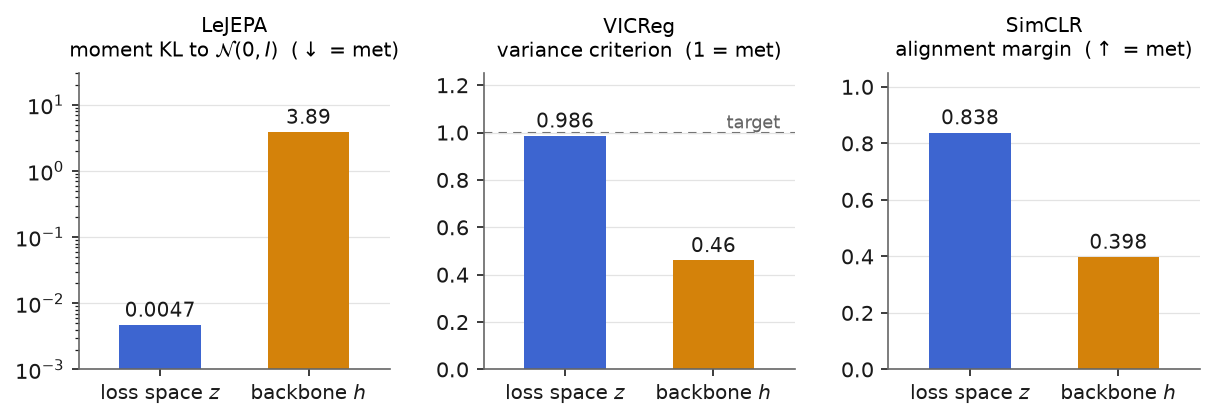
\includegraphics[width=\linewidth]{figures/fig_discrepancy.png}
    \caption{Each method's own training constraint, measured at the loss space $Z$ and at the retained backbone $H$ of the untreated ImageNet-100 models: LeJEPA's moment KL to $\mathcal N(0,I)$ (log scale), VICReg's variance criterion (1 = met), SimCLR's alignment margin. The constraints hold where they are imposed and not at $H$. \BD{THIS GOES TO FIG1 AROUND INTRO?}}
    \label{fig:constraint-mismatch}
\end{figure}
% RAW (not jointly agreed). Source: results/compare/thm21_exhibit.csv; generator fig_discrepancy().

% =========================
% Two-space capacity audit
% =========================
\begin{figure*}[h]
    \centering
    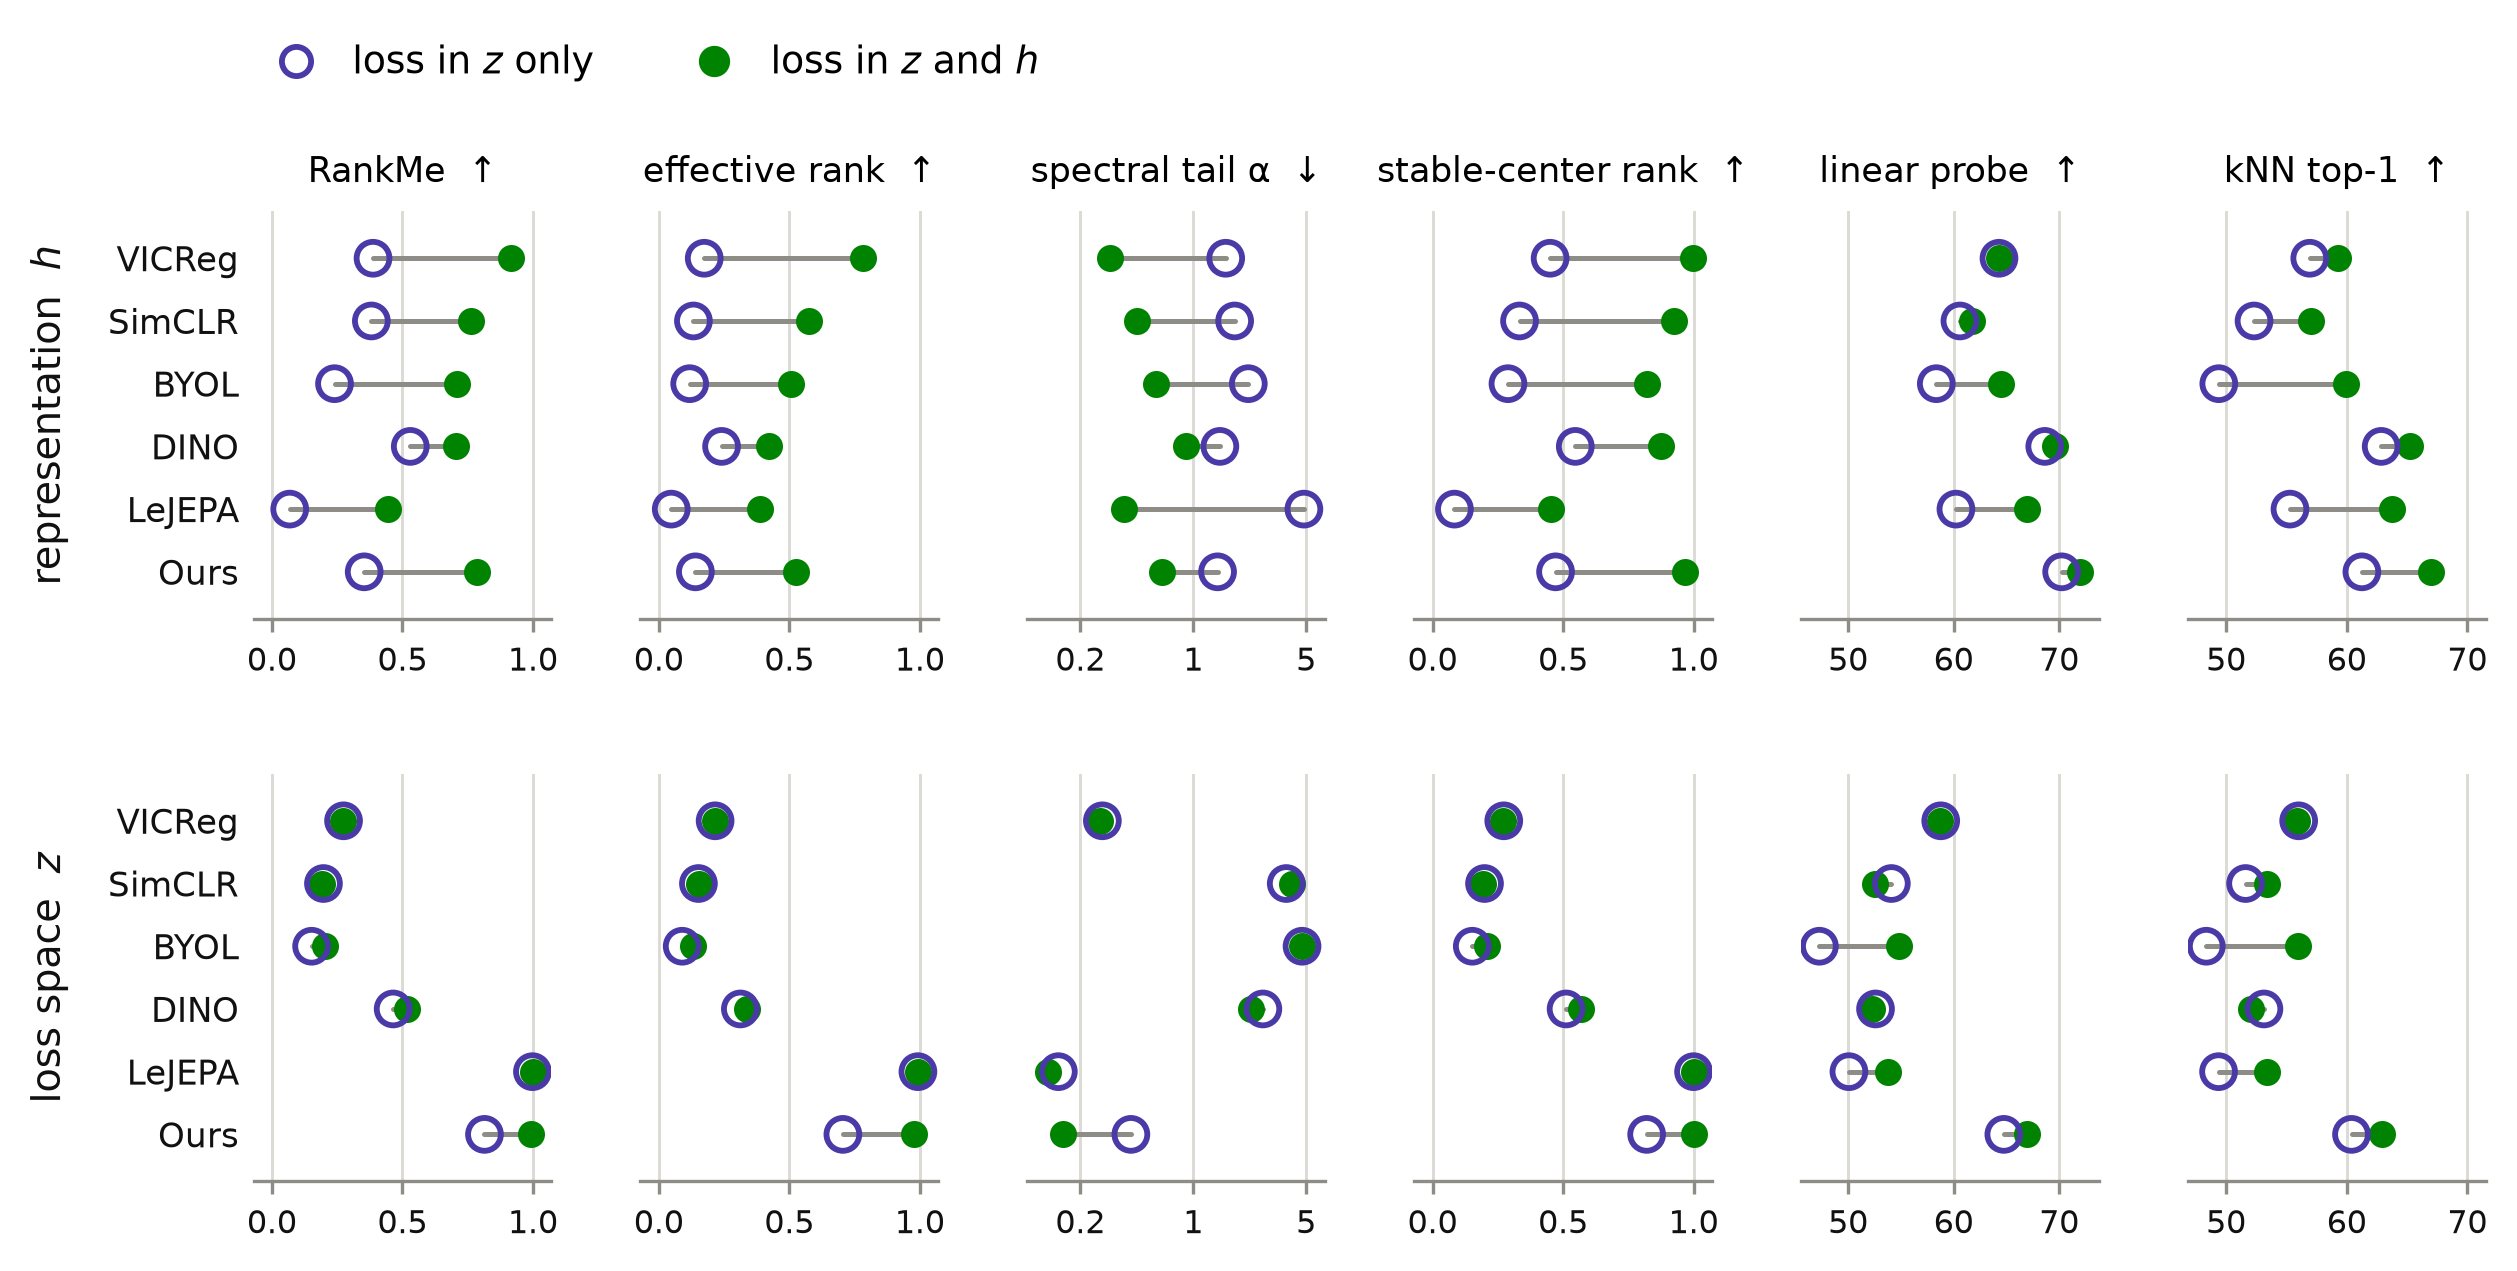
\includegraphics[width=\textwidth]{figures/in100_two_space_audit.png}
    \caption{Effect of the backbone regularizer across six SSL methods on ImageNet-100 (open: loss in $z$ only; filled: loss in $z$ and $h$), measured at the backbone $h$ (top) and after the projector (bottom): RankMe and effective rank over the width, the exponent of the spectral tail, the rank of the stable (between-image) center covariance, and the linear and kNN probes. Backbone capacity and both probes rise for every method; after the projector the statistics move little, except for our own method.}
    \label{fig:two-space-audit}
\end{figure*}
% RAW (not jointly agreed). Source: results/compare/e20_battery_vs_ctrl.csv + results/probes; C2 (AGREED 2026-08-13) for the stable-center rank column.

% =========================
% Accuracy vs augmentation thickness
% =========================
\begin{figure*}[h]
    \centering
    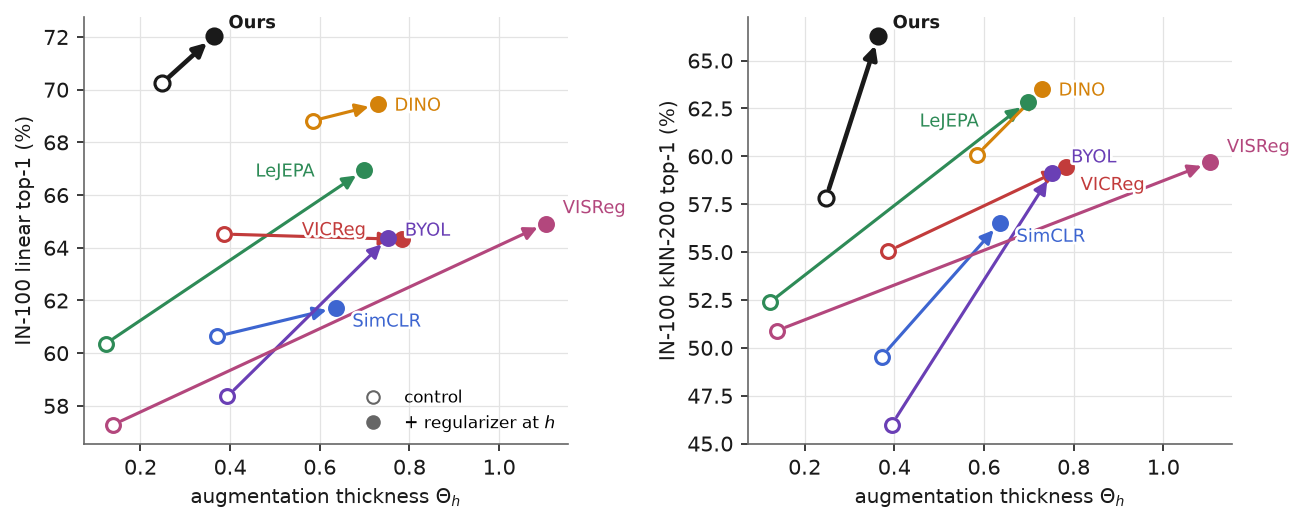
\includegraphics[width=0.82\textwidth]{figures/fig_treatment_arrows.png}
    \caption{Adding the backbone regularizer (open: without; filled: with) makes the backbone representation thicker and more accurate at the same time, for every method: linear probe (left) and kNN (right) against augmentation thickness $\Theta_h$ on ImageNet-100.}
    \label{fig:thickness-gain}
\end{figure*}
% RAW (not jointly agreed). Source: results/diag/e23_retro_spaces.csv (W/B at cls) + results/probes; generator fig_treatment_arrows(). The legend inside the PNG still says "+ moment floor" (retired vocabulary; regenerate).

% =========================
% Organization vs sensitivity
% =========================
\begin{figure*}[h]
    \centering
    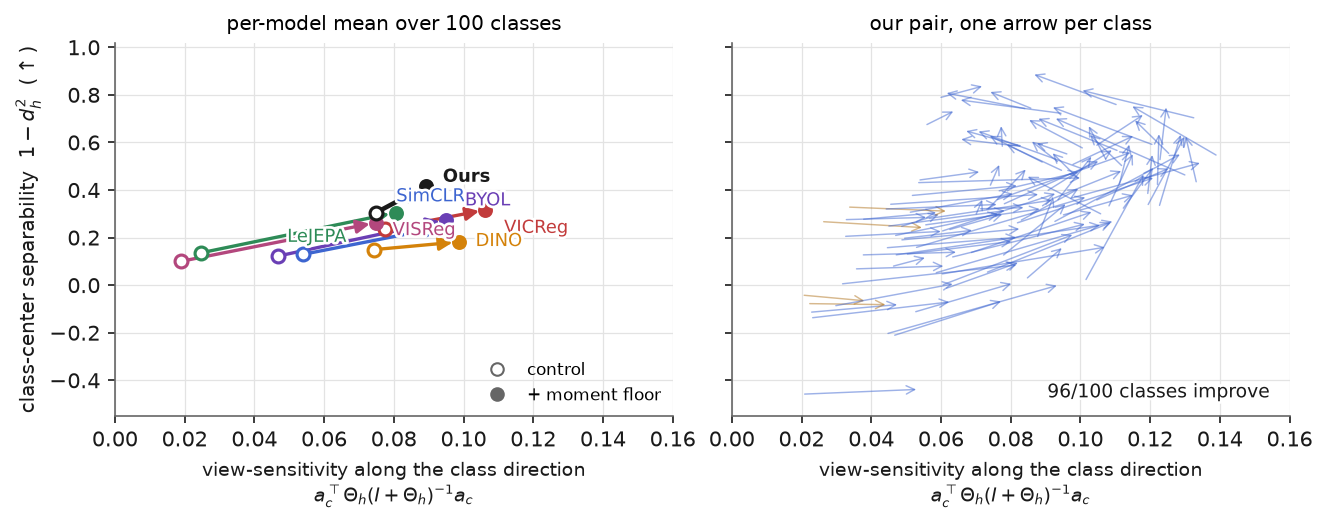
\includegraphics[width=0.85\textwidth]{figures/fig_org_vs_sensitivity.png}
    \caption{The two terms of Eq.~\eqref{eq:too-thick} per class on the ImageNet-100 linear probe: class-center separability $1-d_h^2$ against view sensitivity along the class's own direction, $a_c^\top\Theta_h(I+\Theta_h)^{-1}a_c$. Left: means over the 100 classes for each method (open: without the regularizer; filled: with it). Right: our model, one arrow per class; 96 of 100 move up.}
    \label{fig:organization-sensitivity}
\end{figure*}
% C8, AGREED 2026-08-13 (caption reading = the agreed wording). Source: results/twospace/*.classes.csv; generator fig_org_vs_sensitivity(). Legend inside the PNG: "+ moment floor" (retired vocabulary; regenerate).

% =========================
% Rich feature learning
% =========================
\begin{figure*}[h]
    \centering
    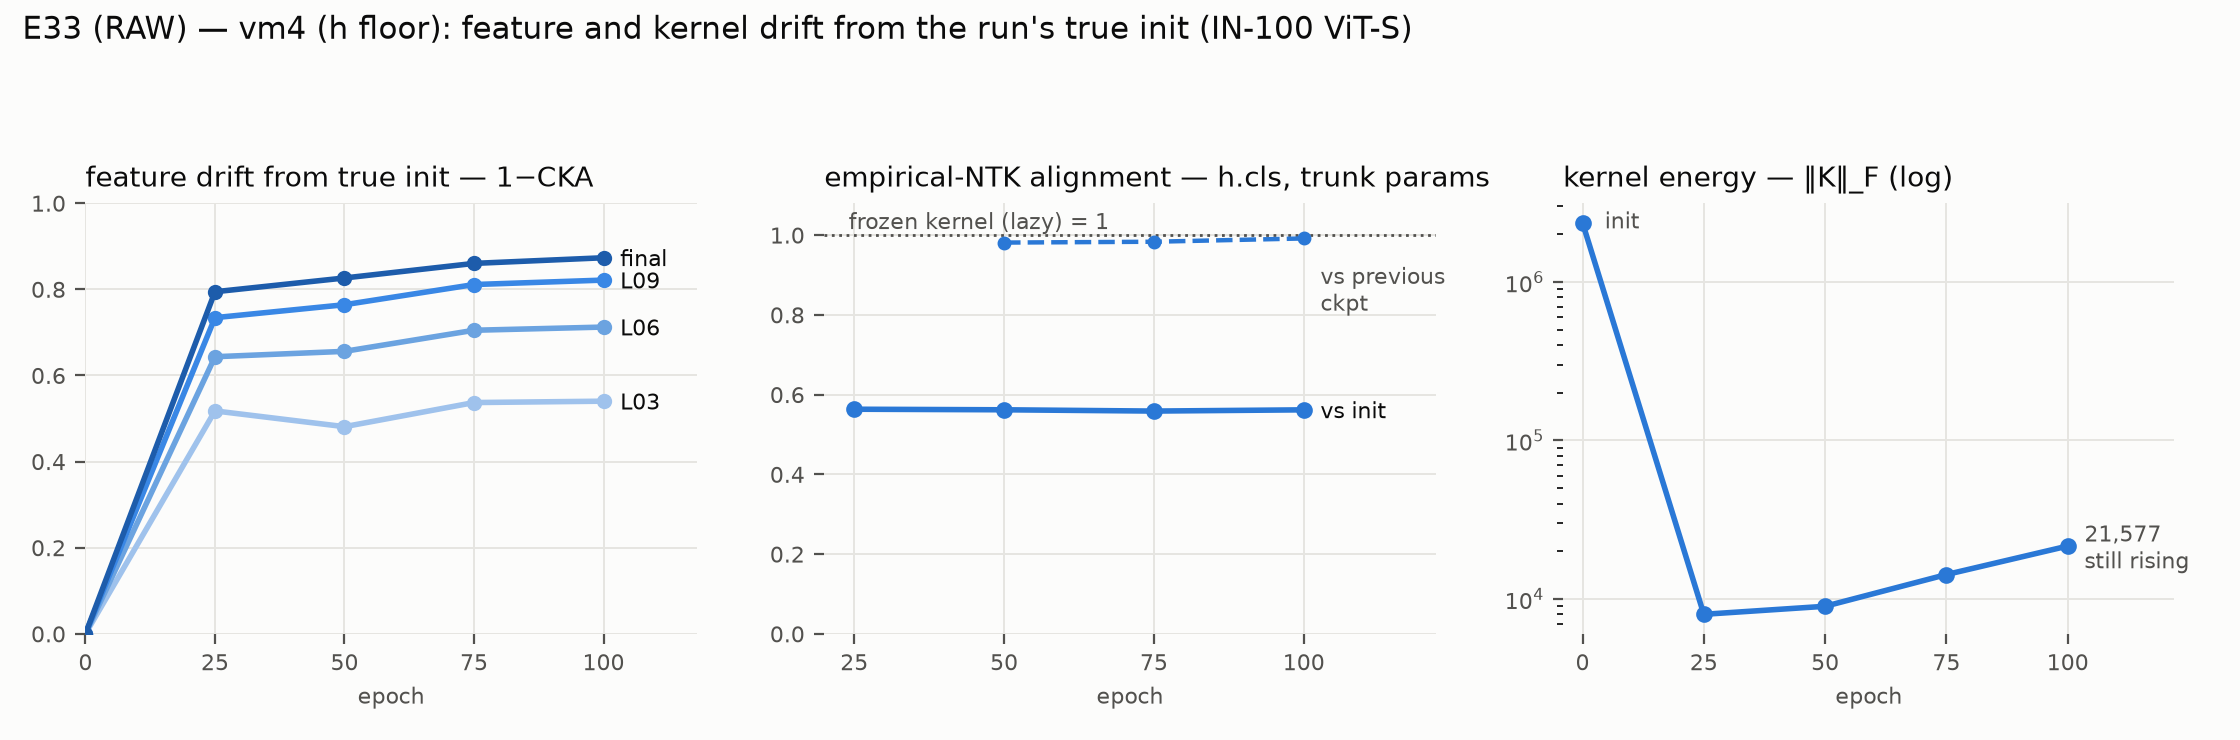
\includegraphics[width=\textwidth]{figures/e33_feature_drift.png}
    \caption{Training with the backbone regularizer stays in the rich regime (ImageNet-100, ViT-S/16). Left: linear-CKA distance of the backbone features from the run's own initialization, per station (final CLS, layers 9 / 6 / 3). Middle: alignment of the empirical tangent kernel (trunk parameters, CLS output) with its initial value; a frozen kernel would read 1. Right: kernel norm over training.}
    \label{fig:rich-learning}
\end{figure*}
% E33-T1, AGREED (D-113). Source: results/diag/feature_drift.in100.floorssl.s0.d256vm4{,zonly}.csv; figure results/figures/e33_feature_drift.png (copied to figures/ 2026-09-15; its title bar still says "E33 (RAW)").

\clearpage
